\section{Tổ chức lưu trữ miền tri thức} 

Tổ chức lưu trữ miền tri thức trong hệ quản trị cơ sở dữ liệu \texttt{(CSDL) MS SQL Server} với các bảng sau:

\begin{itemize}
	\item Bảng \textbf{\texttt{Vertices}}: mỗi dòng định danh đỉnh của đồ thị ($a$, $b$, $c$, $\dots$) với:
	\begin{itemize}
		\item \texttt{id} là dãy số duy nhất cho từng đỉnh, \texttt{name} là tên đỉnh thường được đặt theo ký hiệu toán học.
		\item \texttt{degree} là thuộc tính bậc của đỉnh (${deg_a}$ = 2, ${deg_b}$ = 1 , $\dots$), trong đó một số trường hợp đặc biệt số bậc của đỉnh như ${deg_b}$ = 1, cho biết $b$ là đỉnh treo hay nếu ${deg_b}$ = 0 thì  $b$ là đỉnh cô lập.
	\end{itemize} 
	
	\begin{tabular}{|c|l|}
		\hline
		\multicolumn{2}{|c|}{\textbf{Vertices}} \\
		\hline
		\textbf{PK} & \texttt{\textbf{id int NOT NULL}} \\
		\hline
		& \texttt{name char(50) NOT NULL} \\
		\hline
		& \texttt{degree int NOT NULL} \\
		\hline
	\end{tabular}
	
	\item Bảng \textbf{\texttt{Edges}}: mỗi dòng chứa thông tin của 1 cạnh trong đồ thị bao gồm 2 \texttt{id} của đỉnh từ bảng \texttt{vertices} và độ dài của cạnh.
	
	\begin{tabular}{|c|l|}
		\hline
		\multicolumn{2}{|c|}{\textbf{Edges}} \\
		\hline
		\textbf{FK} & \texttt{\textbf{from\_id char(50) NOT NULL}} \\
		\hline
		\textbf{FK} & \texttt{\textbf{to\_id char(50) NOT NULL}} \\
		\hline
		& \texttt{distance int NOT NULL} \\
		\hline
		& \texttt{name char(100) NOT NULL} \\
		\hline
	\end{tabular}
\end{itemize}
	
Miền tri thức trên cho phép giải các bài toán liên quan tới phân loại đồ thị, tìm đường đi và chu trình đường đi trong đồ thị.

Ví dụ minh họa chi tiết miền tri thức lý thuyết đồ thị bằng cấu trúc bảng dữ liệu với đồ thị gồm 5 đỉnh A,B,C,D,E với độ dài các cạnh tương ứng như bên dưới:

\begin{figure}[h]
	\centering
	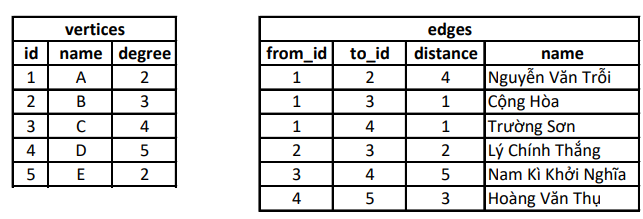
\includegraphics[width= 0.9\linewidth]{tables.PNG}
	\caption{Minh họa miền tri thức định dạng bảng trong CSDL}
	\label{fig-3: dinh dang mien-tri-thuc}
\end{figure}
